%\subsection{Wear the Right Gear}
\langsection[subsection]{Wear the Right Gear}{Правильный экип}

\begin{langblock}{0.425}
	\begin{eng}
	When you ride, your gear is ``right`` if it protects you. In any crash, you have a far better chance of avoiding serious injury if you wear:
	\begin{itemize}[noitemsep]
		\item An approved helmet.
		\item Face or eye protection.
		\item Protective clothing.
	\end{itemize}
	\end{eng}
	\begin{rus}
	
		Когда вы управляете мотоциклом, ваша экипировка является «правильной», если она обеспечивает вам защиту. При любом столкновении у вас значительно больше шансов избежать серьезных травм, если вы используете:
		\begin{itemize}[noitemsep]
			\item Сертифицированный шлем.
			\item Защиту лица или глаз.
			\item Защитную одежду.
		\end{itemize}	
	\end{rus}
\end{langblock}



\begin{figure}[htbp]
	\centering
	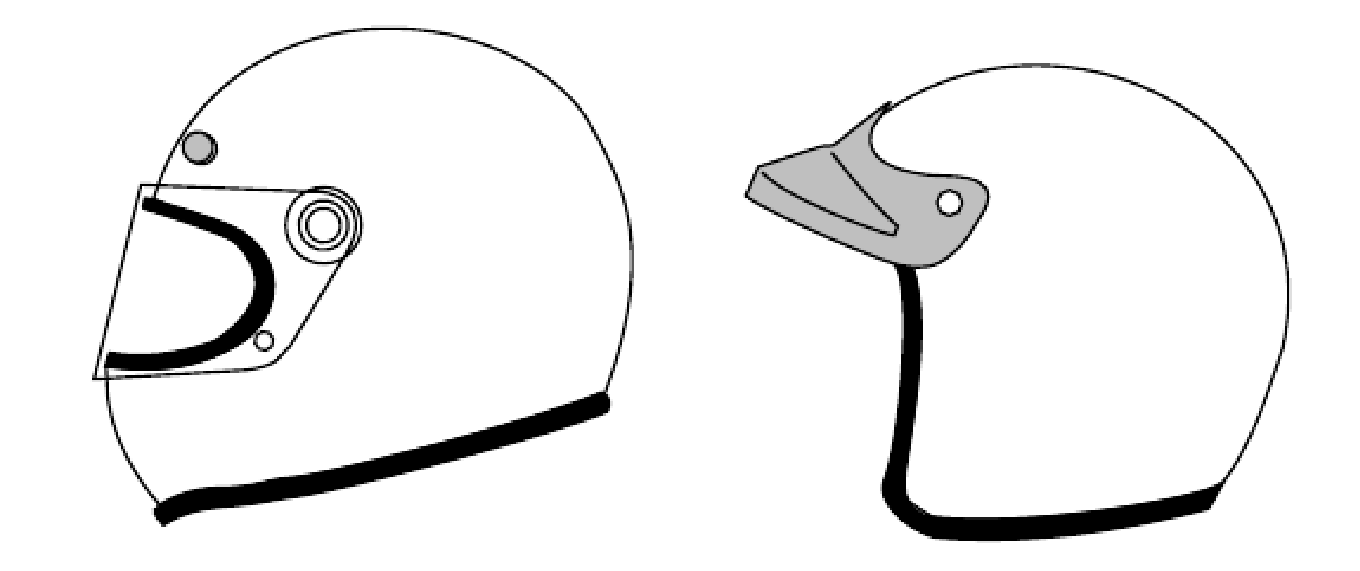
\includegraphics[width=0.95\textwidth, frame]{helmets}
	\caption{Helmets}
	\label{fig:helmets1}
\end{figure}



\langsection[subsubsection]{Helmet Use}{Носите шлем}

\begin{langblock}{0.45} 
	\begin{eng}
	Crashes are not rare events particularly among beginning riders. And one out of every five motorcycle crashes result in head or neck injuries. Head injuries are just as severe as neck injuries and far more common. Crash analyses show that head and neck injuries account for a majority of serious and fatal injuries to motorcyclists. Research also shows that, with few exceptions, head and neck injuries are reduced by the proper wearing of an approved helmet.
	Some riders don't wear helmets because they think helmets will limit their view to the sides. Others wear helmets only on long trips or when riding at high speeds. Here are some facts to consider:
	\begin{itemize}
		\item \textbf{An approved helmet} lets you see as far to the sides as necessary. A study of more than 900 motorcycle crashes, where 40\% of the riders wore helmets, did not find even one case in which a helmet kept a rider from spotting danger.
		\item \textbf{Most crashes happen} on short trips (less than five miles long), just a few minutes after starting out.
		\item \textbf{Most riders} are riding slower than 30 mph when a crash occurs. At these speeds, helmets can reduce both the number and the severity of head injuries by 50\%.
	\end{itemize}
	
	No matter what the speed, helmeted riders are three times more likely to survive head injuries than those not wearing helmets at the time of the crash.
	\end{eng}
	\begin{rus}
		ДТП с мотоциклами не являются редкостью, особенно среди начинающих мотоциклистов. Каждое пятое столкновение с участием мотоцикла приводит к травмам головы или шеи. Травмы головы не уступают по тяжести травмам шеи, однако происходят значительно чаще. Анализ аварий показывает, что травмы головы и шеи составляют большинство серьезных и смертельных травм у мотоциклистов. Исследования также показывают, что за исключением некоторых случаев, надлежащее ношение сертифицированного шлема снижает количество травм головы и шеи. 
		Некоторые мотоциклисты не носят шлемы, поскольку считают, что шлемы ограничивают обзор по сторонам. Другие надевают их только в длительных поездках или при движении на высоких скоростях. Однако, вот несколько фактов о шлемах:
		\begin{itemize}
			\item \textbf{Сертифицированный шлем} обеспечивает обзор по сторонам в необходимом объеме. Исследование более 900 ДТП с участием мотоциклов, в котором 40\% мотоциклистов носили шлемы, не выявило ни одного случая, когда шлем препятствовал обнаружению опасности.
			\item \textbf{Большинство аварий} происходит на коротких маршрутах (протяженностью менее пяти миль) в течение нескольких минут после начала поездки.
			\item \textbf{В момент аварии} большинство мотоциклистов движется со скоростью менее 30 миль в час. При этих скоростях шлемы могут снизить количество и тяжесть травм головы на 50\%.
		\end{itemize}
		Независимо от скорости движения, мотоциклисты в шлемах выживают при травмах головы в три раза чаще по сравнению с теми, кто был без шлема.
	\end{rus}
\end{langblock}


%\subsubsection{Helmet Selection}
\langsection[subsubsection]{Helmet Selection}{Подбор шлема}

\begin{langblock}{0.425} 
	\begin{eng}
	There are two primary types of helmets, providing two different levels of coverage: three-quarter and full face.
	
	Whichever style you choose, you can get the most protection by making sure that the helmet:
	\begin{itemize}
		\item \textbf{Is designed to meet U.S.} Department of Transportation (DOT) and state standards. Helmets with a label from the Snell Memorial Foundation gives you an added assurance of quality.
		\item \textbf{Fits snugly}, all the way around.
		\item \textbf{Has no obvious defects} such as cracks, loose padding or frayed straps.
	\end{itemize}
	Whatever helmet you decide on, keep it securely fastened on your head when you ride. Otherwise, if you are involved in a crash, it's likely to fly off your head before it gets a chance to protect you.
	
	\end{eng}
	\begin{rus}
		Существует два основных типа шлемов, обеспечивающих различные уровни защиты: три четверти и полноразмерные (full face). Какой бы стиль вы ни выбрали, максимальную защиту вы получите при условии, что шлем:
		\begin{itemize}
			\item \textbf{Соответствует стандартам} Министерства транспорта США (DOT) и требованиям штата. Шлемы с маркировкой Snell Memorial Foundation обеспечивают дополнительную гарантию качества.
			\item \textbf{Обеспечивает плотную посадку} по всей окружности.
			\item \textbf{Не имеет явных дефектов}, таких как трещины, ослабление прилегания или изношенные ремни.
		\end{itemize}
		Каким бы шлемом вы ни воспользовались, всегда надежно закрепляйте его на голове. В противном случае, он, вероятно, слетит с головы раньше, чем успеет вас защитить.
\end{rus}
\end{langblock}



\langsection[subsubsection]{Eye and Face Protection}{Защита для глаз и лица}

\begin{langblock}{0.425} 
	\begin{eng}
	A plastic shatter-resistant faceshield can help protect your whole face in a crash. It also protects you from wind, dust, dirt, rain, insects, and pebbles thrown up from cars ahead. These problems are distracting and can be painful. If you have to deal with them, you can't devote your full attention to the road.
	
	Goggles protect your eyes, though they won't protect the rest of your face like a faceshield does. A windshield is not a substitute for a faceshield or goggles. Most windshields will not protect your eyes from the wind; neither will eyeglasses or sunglasses. Glasses won't keep your eyes from watering, and they might blow off when you turn your head while riding.
	
	\textit{To be effective, eye or faceshield protection must:}
	\begin{itemize}[noitemsep]
		\item \textbf{Be free} of scratches.
		\item \textbf{Be resistant} to penetration.
		\item \textbf{Give a clear} view to either side.
		\item \textbf{Fasten securely}, so it does not blow off.
		\item \textbf{Permit air} to pass through, to reduce fogging.
		\item \textbf{Permit enough room} for eyeglasses or sunglasses, if needed.
	\end{itemize}
	Tinted eye protection should not be worn at night or any other time when little light is available.
	
	\end{eng}
	\begin{rus}
		Пластиковый небьющийся визор (faceshield) способен защитить все лицо при аварии. Он также защищает от ветра, пыли, грязи, дождя, насекомых и камней, вылетающих из-под автомобилей. Это не только отвлекает внимание, но и может травмировать. Защитные очки (goggles) защищают глаза, однако они не защищают остальное лицо так как это делает визор. Ветровое стекло (windshield) мотоцикла не заменяет визор или защитные очки. Большинство ветровых стекол не защищают глаза от ветра; обычные или солнцезащитные очки также не обеспечивают такой защиты. В обычных очках глаза могут слезиться, а еще они могут слететь при повороте головы. Чтобы защита глаз или визор были эффективны, они должны:
		\begin{itemize}[noitemsep]
			\item \textbf{Не иметь царапин}.
			\item \textbf{Быть устойчивыми} к пробитию.
			\item \textbf{Обеспечивать четкий обзор} по сторонам.
			\item \textbf{Надежно крепиться}, чтобы их не сдуло ветром.
			\item \textbf{Пропускать воздух} для предотвращения запотевания.
			\item \textbf{Предоставлять достаточное пространство} для очков или солнцезащитных очков при необходимости.
		\end{itemize}
		Тонированные средства защиты глаз не следует использовать в темное время суток или в любых условиях недостаточной освещенности.
	\end{rus}
\end{langblock}


\langsection[subsubsection]{Clothing}{Одежда}
\begin{langblock}{0.425} 
	\begin{eng}
	The right clothing protects you in a collision. It also provides comfort, as well as protection from heat, cold, debris, and hot and moving parts of the motorcycle. It can also make you more visible to others.
	\begin{itemize}
		\item \textbf{Jacket and pants} should cover arms and legs completely. They should fit snugly enough to keep from flapping in the wind, yet loosely enough to move freely. Leather offers the most protection. Sturdy synthetic material provides a lot of protection as well. Wear a jacket even in warm weather to prevent dehydration. Many are designed to protect without getting you overheated, even on summer days.
		\item \textbf{Boots or shoes} should be high and sturdy enough to cover your ankles and give them support. Soles should be made of hard, durable slip resistant material. Keep heels short so they do not catch on rough surfaces. Tuck laces in so they won't catch on your motorcycle.
		\item \textbf{Gloves} allow a better grip and help protect your hands in a crash. Your gloves should be made of leather or similar durable material.
	\end{itemize}
	In cold or wet weather, your clothes should keep you warm and dry, as well as protect you from injury. You cannot control a motorcycle well if you are numb. Riding for long periods in cold weather can cause severe chill and fatigue. A winter jacket should resist wind and fit snugly at the neck, wrists, and waist. Good-quality rainsuits designed for motorcycle riding resist tearing apart or ballooning up at high speeds.
	\end{eng}
	\begin{rus}
		Правильная одежда защищает вас при столкновении. Она также обеспечивает комфорт и защиту от жары, холода, мусора, а также от горячих и подвижных деталей мотоцикла. Кроме того, она повышает вашу заметность.
		\begin{itemize}[nosep]
			\item \textbf{Куртка и брюки} должны полностью закрывать руки и ноги. Они должны сидеть достаточно плотно, чтобы не развеваться на ветру, но достаточно свободно, чтобы не стеснять движений. Кожа обеспечивает наибольшую защиту. Прочные синтетические материалы также обеспечивают значительную защиту. Надевайте куртку даже в теплую погоду для предотвращения обезвоживания. Многие модели разработаны таким образом, чтобы защищать, не вызывая перегрева даже в летние дни.
			\item \textbf{Ботинки или обувь} должны быть достаточно высокими и прочными, чтобы закрывать голеностопные суставы и обеспечивать им поддержку. Подошвы должны быть изготовлены из твердого, долговечного нескользящего материала. Каблуки должны быть короткими, чтобы не цепляться за неровные поверхности. Заправляйте шнурки, чтобы они не зацепились за мотоцикл.
			\item \textbf{Перчатки} обеспечивают более надежный хват и помогают защитить руки при аварии. Перчатки должны быть изготовлены из кожи или аналогичного прочного материала.
		\end{itemize}
		В холодную или влажную погоду одежда должна сохранять тепло и сухость, а также защищать от травм. Вы не сможете рулить, если у вас затекут конечности. Длительная езда в холодную погоду может вызвать сильное переохлаждение и усталость. Зимняя куртка должна быть ветронепроницаемой и плотно прилегать в области шеи, запястий и талии. Качественные дождевики, предназначенные для езды на мотоцикле, устойчивы к разрывам и раздуванию на скорости.
\end{rus}
\end{langblock}



